L'analyse sémantique du Stibbons est effectué dans les classes Interpreter. Plus exactement dans 3 classes (cf UML~\ref{interpreterUML} page~\pageref{interpreterUML}).

\begin{figure}[h]
\caption{\label{interpreterUML} UML de l'analyseur sémantique}
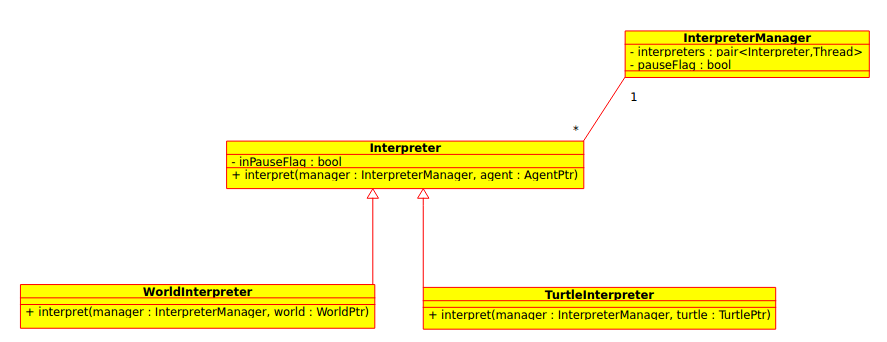
\includegraphics[scale=0.5]{doc/report/uml/interpreterUML.png}
\end{figure}

On a donc les classes \verb|TurtleInterpreter| et \verb|WorldInterpreter| qui héritent de la classe \verb|Interpreter|. Cette dernière analyse et provoque, dans le modèle, les actions liées au code stibbons écrit. Elle permet de gérer tout type d'interaction, du moment que ces actions ne sont pas liées à un monde ou à une tortue. La classe \verb|TurtleInterpreter| gère justement ce dernier type d'actions : celles liées à une tortue. Contrairement à \verb|WorldInterpreter| qui gère les actions du monde.

L'utilité de la classe \verb|InterpreterManager| est expliqué de manière détaillée dans la section \ref{remaniementInterpreter} (page~\pageref{remaniementInterpreter}).

Ainsi, pour avoir un exemple concret, si on demande à une tortue d'avancer en Stibbons (ex : \verb|fd 10|), alors c'est le \verb|TurtleInterpreter| qui gèrera cette action.
A contrario, si on effectue une définition de fonction (ex : \verb|a = 10|) alors l'\verb|Interpreter| affectera la valeur \verb|10| à la propriété \verb|a| de l'agent courant.
Pour ce qui est du WorldInterpreter, il n'y a pas encore d'exemple possible, tout simplement car pour l'instant il n'y a pas d'actions spéciales pour le monde.

\subsection{Fonctionnalités}

\subsubsection{Sprint 1 \& 2}
Les deux premiers sprints ont été assez conséquent au niveau du nombre de fonctionnalités ajoutées.
En effet lors du sprint 1, on pouvait déjà effectuer les opérations de bases sur une tortue, telles que avancer, tourner, écrire, etc. De plus les opérations de calcul ainsi que la gestion de nombres ont été fait. En effet, il était nécessaire de gérer les nombres de manière à pouvoir indiquer à la tortue de quelle distance elle devait avancer.

Lors du deuxième sprint sont apparu les conditionnelles, ainsi que les boucles, les comparaisons binaires, les booléens et autres types (color, string, etc.), la création de nouveaux agents dans le code et les fonctions sans paramètres. Ce sprint fut alors une version déjà bien avancée de notre programme final.


\subsubsection{Sprint 3 à 5}
Les sprints suivants ont été plus léger. Non pas parce qu'il y avait moins de travail, car la gestion de l'interpréteur fut remanier à ce moment là, mais car il y avait moins de fonctionnalités à ajouter. En effet, à partir du sprint 3, les fonctionnalités suivantes ont été rajoutés~:
\begin{itemize}
\item accès à la parenté et aux zones (en lecture seulement)~;
\item ajout des tables et de boucles dédiés (\verb|foreach|)~;
\item gestion de la vitesse et de la pause~;
\item ajout des communications avec le \verb|send| et le \verb|recv|.
\end{itemize}


\subsection{Fonctionnement}
Lors de l'analyse d'un jeton, qui correspond à un noeud de l'arbre syntaxique, on analyse d'abord ses fils (s'il y en a) puis ensuite le contenu du noeud actuel.
Ainsi pour le test d'égalite \verb|1 == 2|, le noeud \verb|==| aura pour enfants les sous-arbres de noeud \verb|1| et \verb|2| qui seront analysés en premier. Puis le test \verb|==| sera appliqué sur le résultat de l'analyse de ces deux noeuds.
Certains cas sont plus compliqués, comme lors de l'affection où, une fois le résultat des noeuds obtenus, une vérification de l'existance de la variable affectée est faite sur l'agent parent. Si la variable existe déjà, elle hérite de la valeur affecté dans le parent, sinon elle est égale à \verb|null|.
Par exemple, dans le listing ~\ref{affect-parent}, la variable b existe dans wolf car son parent, le monde, possède une variable b égale à 2. Or dans le listing ~\ref{non-affect-parent} la variable b n'existe pas dans le monde, elle n'est pas non plus initialisé dans wolf, donc elle est égale à \verb|null|.

\begin{lstlisting}[label=affect-parent,caption=Affectation d'une variable héritée]
b = 2
agent wolf(){
	println(parent.b)
}
new wolf()
\end{lstlisting}
\begin{lstlisting}[label=non-affect-parent,caption=Erreur d'affectation d'une variable héritée]
agent wolf(){
	println(parent.b)
}
new wolf()
\end{lstlisting}

Un autre cas complexe est celui de la création d'un nouvel agent. Ici on crée n nouveaux agents d'un certain type, explicité(\verb|n new nomBreed()|) ou anonyme(\verb|n new agent|). Ces nouveaux agents vont~:
\begin{itemize}
\item récupérer le code correspondant à leur type (la \verb|breed|)~;
\item charger leurs paramètres, seulement si la breed n'est pas anonyme~;
\item être lancés dans un thread.
\end{itemize}


\subsection{Remaniement de l'analyseur sémantique}
\label{remaniementInterpreter}

L'analyseur sémantique a d'abord été une seule classe~: la classe \verb|Interpreter|.
Cette dernière implémentait tout types d'actions à effectuer pour n'importe quel type d'agent.
Cependant, lors de l'arrivée de la fonctionnalité d'ajout d'un nouvel agent (\verb|new agent|), nous nous sommes aperçu qu'il serait mieux d'avoir un interpréteur par type d'agent, ou plus précisement un interpréteur pour le monde, un pour les tortues et un pour les actions communes aux deux types.
Nous avons alors crée les deux classes~: \verb|WorldInterpreter| et \verb|TurtleInterpreter|.

De manière parallèle, la création du monde s'effectuait dans l'\verb|Interpreter|, puis dans le \verb|WorldInterpreter|, il fut alors nécessaire de créer une classe qui gérerait à la fois la création du monde et tout ce qui concernait l'application (la pause, le temps, les interpreteurs eux-mêmes). Nous avons alors décidé de créer la classe \verb|InterpreterManager|.
Cette classe connait tous les interpréteurs, et permet de les prévenir d'une éventuelle pause du programme, de stocker les threads correspondants à chaque interpréteur, de créer un monde avec les pré-directives choisies~; c'est une sorte de gestionnaire d'interpréteurs.
